\section{Startup Workspace} \label{startup_workspace}
\label{section:startup_workspace}

It has already been mentioned that the startup workspace is loaded when you start \Voreen for the first time. Later, \Voreen
will always load the last workspace you worked with when starting the application. If you need to open the
startup workspace at a later time, it can be found under:
\begin{center}
\begin{tabular}{|c|} \hline
\verb|resource|\textbackslash\,\verb|voreenbiology|\textbackslash\,\verb|workspaces|\textbackslash\,\verb|startup.vws| \\ \hline 
\end{tabular}
\end{center}
After you have configured the basic application settings described in section \ref{section:configuration}, the 
startup workspace is a good way to get familiar with the basic interface of \Voreen. 
The workspace has already been shown in figure \ref{fig:vb_complete_interface} on page \pageref{fig:vb_complete_interface}. 
In the following description it is assumed that you are familiar with the documentation of section \ref{getting_started}.
  
\subsection{Quad View}

In the quad view of the startup workspace, only two of the four views actually offer interactive functionality. In the top left
view, a three-dimensional rendering of an example data set is displayed, while the bottom right view contains a two-dimensional slice
view. All of the interaction possibilities described in section \ref{section:quadview} are available in those two views, including
the double-click function to enlarge any of the four views. We recommend that you take some time to get used to the quad view controls
before moving on to the other sections.

\subsection{Available Properties}

The startup workspace only contains a small number of properties which are available to the user. If you look at the property window 
at the right side of the application, you will see two groups. The first one contains the color map. In this workspace, the color map
of the three-dimensional view and the slice view is linked, so that only one color map property is present in the workspace. You should 
take some time to get familiar with the color map property and its functionality. Please refer to section \ref{section:color_map} for more
information on how to use color map properties.

The second group, which is called \emph{2D Slice Options}, refers to the slice view at the bottom right of the quad view. If you open the
group it should look similar to figure \ref{fig:startup_property}.

\begin{figure}[h]
 \centering
 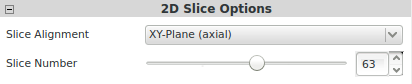
\includegraphics[scale=0.85,keepaspectratio=true]{./images/startup_property.png}
 % startup_property.png: 412x84 pixel, 72dpi, 14.53x2.96 cm, bb=0 0 412 84
 \caption{The slice view property group of the startup workspace}
 \label{fig:startup_property}
\end{figure}

This allows to select the slice alignment of the slice viewer and to change the slice number currently displayed in the bottom right of the 
quad view. You should notice that changing both the slice alignment and the slice number will not only have an effect on the slice view
in the bottom right, but also on the three-dimensional
image in the quad view, where the position of the current slice is marked by colored lines.

The property list window of the startup workspace offers a third property group, which is called \emph{2D Slice Options}. This group
provides the control elements for a single arbitrarily oriented clipping plane. For more information on how to use the clipping plane,
please refer to section \ref{section:clipping_planes}. Please note that the clipping plane only affects the three-dimensional view,
not the two-dimensional slice view.

\subsection{Animation}

Section \ref{section:animation_editor} has been considered with the animation editor of \Voreen. It has already been mentioned that 
the startup workspace already contains an example animation. When opening the animation editor in the startup workspace, it should look
similar to figure \ref{fig:startup_animation}.

\begin{figure}[htb]
 \centering
 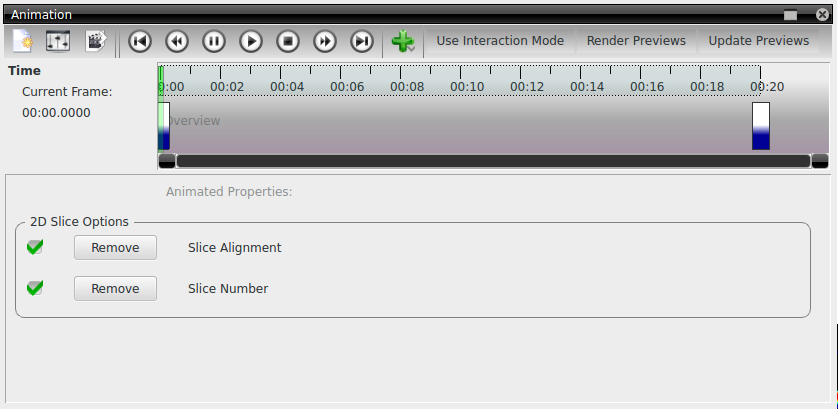
\includegraphics[scale=0.5,keepaspectratio=true]{./images/startup_animation.png}
 % startup_animation.png: 838x409 pixel, 72dpi, 29.56x14.43 cm, bb=0 0 838 409
 \caption{The example animation in the startup workspace}
 \label{fig:startup_animation}
\end{figure}

You should see that two keyframes have been added to the animation, one at the beginning and one at the end. Two of the properties
available in the startup workspace have been animated, the slice alignment and the slice number. The animation simply sets the slice 
alignment to the $xy$-plane and scans through all the slices. This is done by setting the slice number in the first keyframe to $0$ 
and the slice number in the second keyframe to the maximum. The default linear interpolation between the two slice numbers will do the rest.
Try to playback the animation using the playback control icons and watch the changes in the quad view (and in the property list window,
if you have opened the slice options property group). You can move the keyframes in the animation, change the values of the keyframes,
or add the color map property to the list of animated properties. You can also export the animation as a video file or create a completely
new animation. If you want to reset all your changes, simply load the startup workspace again.


\newpage